\chapter{Introduction}
\label{chap:intro}
\section{Motivations}
To all but the dinosaurs, meteors are quite cool. I must first admit that I have lied to you: this report is not about why meteors rock. In fact, half of meteors {\it aren't} made of rock, but it got your attention, didn't it? And now you're reading this! In this report I provide an analysis of a variety of variables that apply to meteor detection. Each of these analyses has it's own significance purely based on knowledge, though I have decided to venture into this EMC project out of my own interest in the subject. Much of the work in this report has been an intention of mine for a year or two; as a product of working with colleagues that are now very much my friends in the Lockyer Technology Centre (LTC) at the Norman Lockyer Observatory (NLO).
\section{Background}
\subsection{What is a meteor?}
Meteoroids are rocky or metallic bodies much smaller than asteroids, which, despite sizes ranging from a grain of sand to centimetres wide, produce streaks of light from the intense heat vaporising the meteoroid. At this point, it is a meteor. It is a matter of debate whether the meteor is the object causing the streak across the sky, or the streak itself. Meteors that survive the plummet to Earth are promoted to meteorites. \\
\subsection{Radio meteor detection}
The intense heat of a meteor ionises the air around it, causing the visible streak seen in the sky. The ionised air along the path of the meteor is capable of reflecting radio waves, allowing a signal to be received. This is radio meteor detection. The diagram for detection is shown in figure~\ref{fig:detection}. 
\begin{figure}
	\centering
	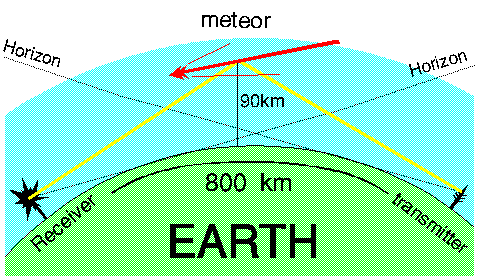
\includegraphics[width=\linewidth]{intro/detection}
	\caption{Diagram of forward scatter radio meteor detection (courtesy of \cite{forwardscatter})
		\label{fig:detection}}
\end{figure}\\
The transmitting antenna sends out a signal that reflects off of the ionised trail and is received by another station. The data that comes from detecting these ionised trails can be considered in various ways; most popularly by simply counting the number of detections an hour, or more visibly by displaying the intensity of the reflected signal for a range of frequencies against time. This produces a rather beautiful `waterfall' plot, seen in figure~\ref{fig:waterfall}. 
\begin{figure}[h!]
	\centering
	\begin{subfigure}{.24\textwidth}
		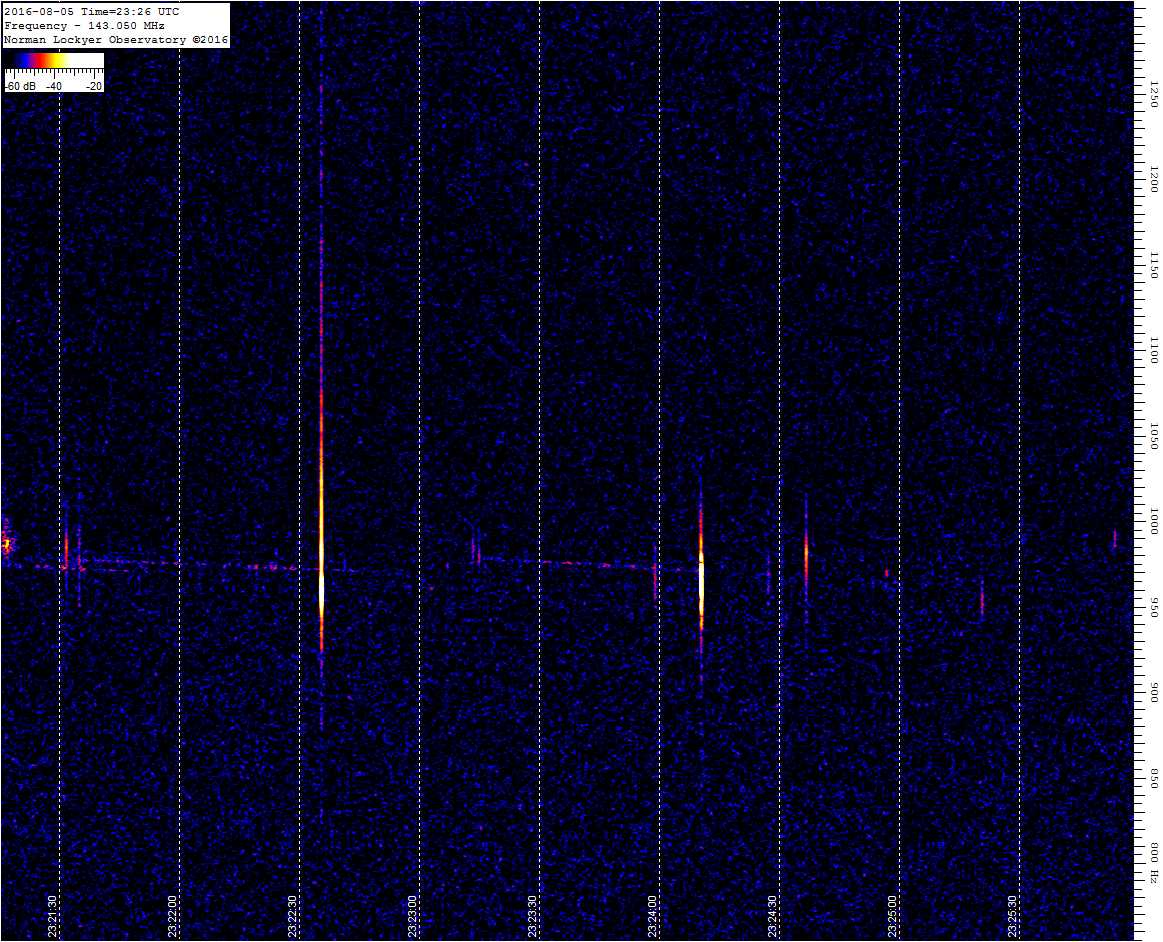
\includegraphics[width=\textwidth]{intro/2D}
		\caption{2D\label{fig:waterfall:a}}
	\end{subfigure}
	\begin{subfigure}{.24\textwidth}
		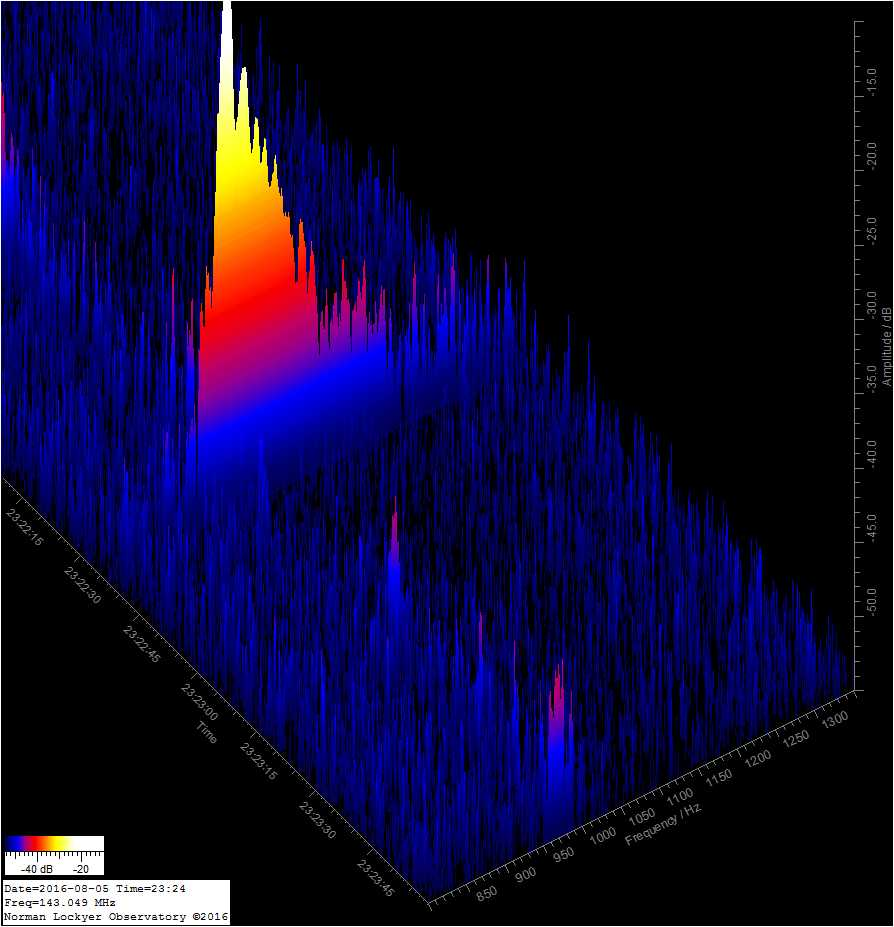
\includegraphics[width=\textwidth]{intro/3D}
		\caption{3D \label{fig:waterfall:b}}
	\end{subfigure}
	\caption{Waterfall plot 
	\label{fig:waterfall}}
\end{figure}\\
The `echo' received from the meteor has a characteristics shape depending on whether upper sideband (USB) or lower sideband (LSB) is used. In figure~\ref{fig:waterfall:a}, USB is used, producing an echo that trails off to the right, and has a peak to the left. The colour of the peak indicates the intensity of the received echo. The blue noise surrounding the echo is radio noise.\\
The alternative method, counting the number of meteors detected in an hour, is discussed in chapter~\ref{chap:data}.

\subsection{Meteor showers}
Typically, visual observation of meteors is done during a meteor shower. This event is characterised by an increased number of meteors observed, that are not sporadic. Sporadic meteors are those that do not appear to come from a common source -- they are simply debris entering the Earth's atmosphere. During a meteor shower, many more meteors are observed than normal, and most importantly, they appear to come from a common source: the radiant. This is the {\it apparent} source of all the shower meteors, that is, the meteors appear to travel out in all directions from this point.\\
The cause of a meteor shower is the Earth passing through the trail of debris left by a comet: dirty snowballs (figure~\ref{stream}). The only (notable) exception to this is the Geminids shower, which is caused by a Palladian asteroid rather than a comet's trail \cite{palladian}. The debris can be produced in many different ways, either through water vapour drag \cite{watervapour} (cite Fred Whipple 1951), by which ice melts and drags sand and pebble sized debris off the comet, or the breakup of parts of a comet.\\
\begin{figure}[h!]
	\centering
	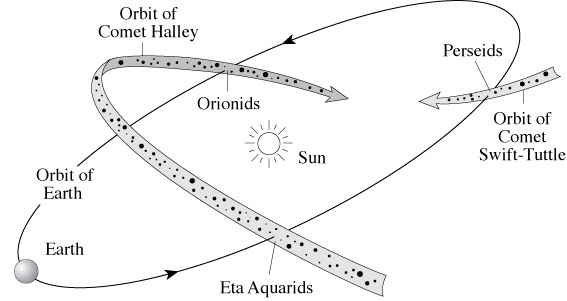
\includegraphics[width=\linewidth]{intro/stream}
	\caption{Meteor stream diagram (courtesy of \cite{stream})}
\end{figure}\\
As time passes, the stream will pass around the Sun and spread out. This means that, with time, a meteor shower's peak will become less pronounced as the meteoroids spread out across the entire orbit of the debris. However, showers caused by periodic comets will not suffer this effect since with each of the Comet's orbits, more debris is shed.\\
\begin{figure}
	\centering
	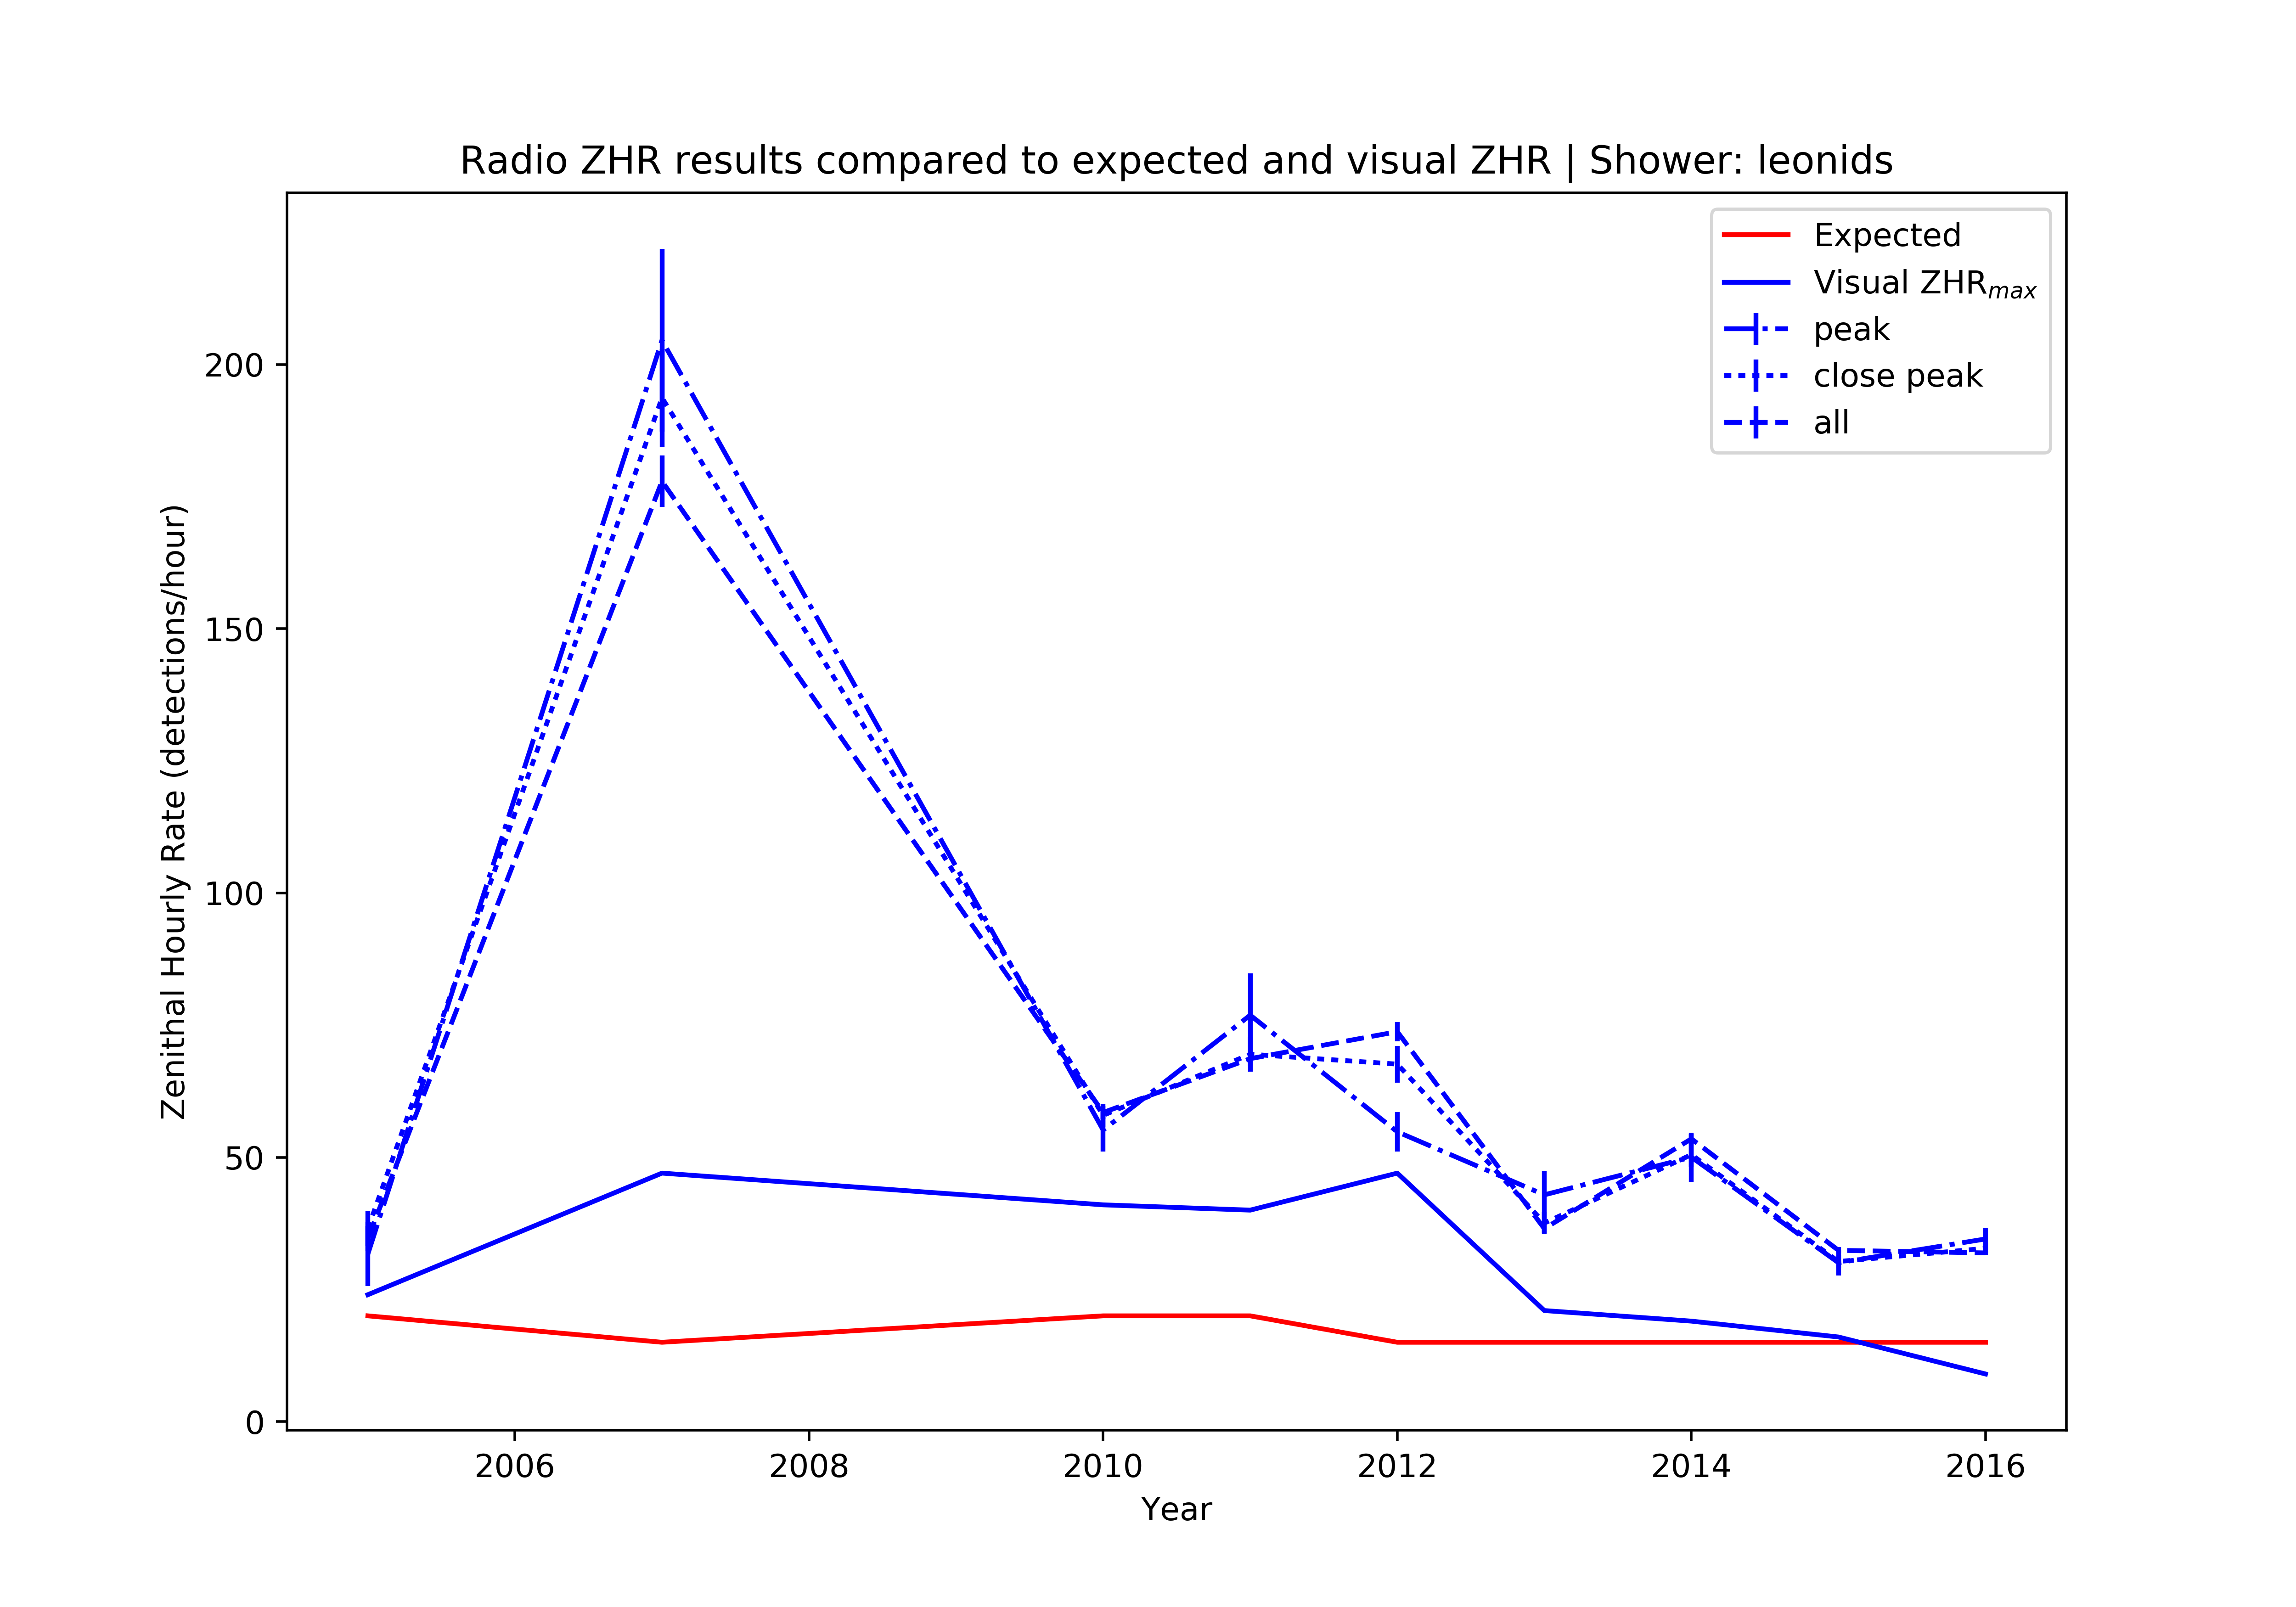
\includegraphics[width=0.8\linewidth]{intro/leonids}
	\caption{Leonids shower November 1833 (courtesy of \cite{leonids}) 
		\label{fig:1833leonids}}
\end{figure}\\
The most famous meteor showers include the Perseids, which often have the greatest number of meteors observed, which peak on the 12th or 13th of August. The Leonids originally gave birth to the name `meteor shower',  after a meteor `storm' in 1833 producing thousands of meteors a minute. (figure~\ref{fig:1833leonids}) This occurs once every 33 years (on average). Other showers, such as the Taurids, do not produce as many meteors, but are notable for frequent fireballs. These are meteors that explode due to the incredible pressure and heat of re-entry, and cause a sudden flash of light that can often illuminate the whole sky.


\subsection{Magnitude}
A measure of brightness (used throughout Astronomy) is magnitude. The magnitude scale is logarithmic and historically based around a single star, $\alpha$ Lyrae, which was used as the 0 point, though it is now defined in terms of flux. A decrease in magnitude by 1 means a brightness increase of $\sqrt[5]{100} \approx 2.512$. The larger the magnitude of a star, the fainter it is. Negative magnitudes are possible: for example, the Sun has an apparent magnitude of -27.\\
Apparent magnitudes are a measure of brightness from Earth, whilst absolute magnitudes are an objective measure of brightness, being the theoretical brightness of a star from a set distance (1 parsec). For visual observation (naked eye), meteors fainter than 6.5 in apparent magnitude cannot be seen. This is not the case for radio meteor detection.